%! Author = antonio
%! Date = 7/2/24

Multivariate Gaussian Density is an extension of the Gaussian Density to multiple dimensions.
It is used to describe the distribution of a vector of random variables in a \(multi-dimensional\) space,
and it could be defined as:
\begin{equation}
    N(x\mid\mu, \Sigma) = \frac{1}{(2\pi)^{\frac{M}{2}} \left|\Sigma \right|^{\frac{1}{2}}}\exp^{-\frac{1}{2}(x-\mu)^T\Sigma^{-1}(x-\mu)}
    \label{eq:gaussianDensity}
\end{equation}

where \(M\) is the size of the feature vector \(x\), and \(\left|\Sigma \right|\) is the determinant of \(\Sigma\).
Since the computation of the exponential could cause problems, the logarithm is applied, so from \autoref{eq:gaussianDensity}
we get \autoref{eq:logGaussianDensity}:

\begin{equation}
    \log N(x\mid\mu, \Sigma) = -\frac{M}{2}\log(2\pi) - \frac{1}{2}\log\left|\Sigma \right| - \frac{1}{2}(x-\mu)^T\Sigma^{-1}(x-\mu)
    \label{eq:logGaussianDensity}
\end{equation}

\begin{figure}[h]
    \centering
    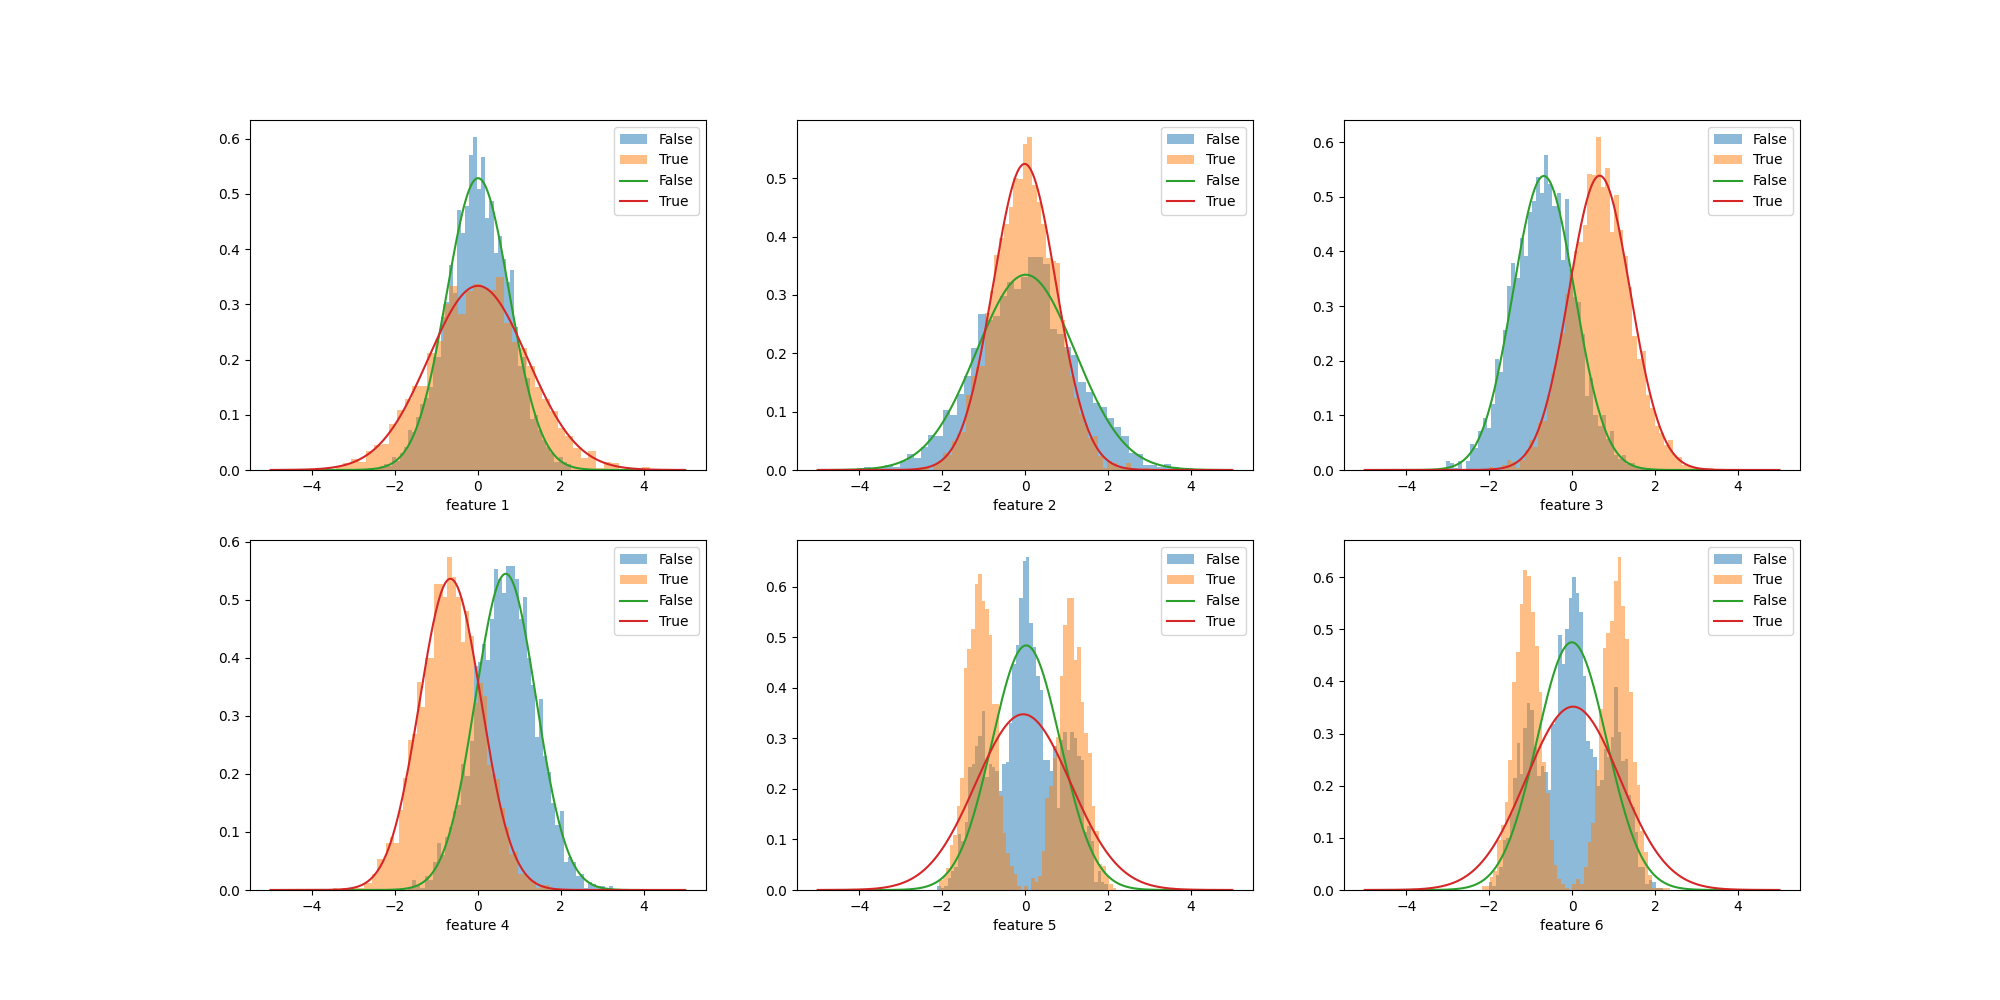
\includegraphics[width=1\linewidth]{Lab/04. Lab 04/Images/01. GaussianDensity}
    \caption{Gaussian Density}
    \label{fig:gaussianDensity}
\end{figure}

Thus, applying Gaussian probability density to the 6 features in our dataset, the following results in \autoref{fig:gaussianDensity},
are obteinded.\\
It can observe that \textbf{features 1 - 2 - 3 - 4} fit the Gaussian distribution,  the histogram of the data is well
approximated by the Gaussian curve.
For \textbf{features 5 - 6} this does not happen and therefore could not be a good model.